\documentclass{article}
\usepackage{amsthm}
\usepackage{amsmath}
\usepackage{graphicx}
\usepackage{multirow}

\newtheorem{problem}{Problem}

\begin{document}
\title{Bit Sets}
\author{Henry Z. Lo}
\maketitle

\section{Set Operations}
Common operations on sets include:
\begin{enumerate}
\item Union (or): what is in either one or both of the sets.
\item Intersection (and): what is in both sets.
\item Symmetric difference (xor): what is in one, but not both sets.
\item Subtraction: what is in the first set, but not the second.
\end{enumerate}

\begin{figure}
\centering
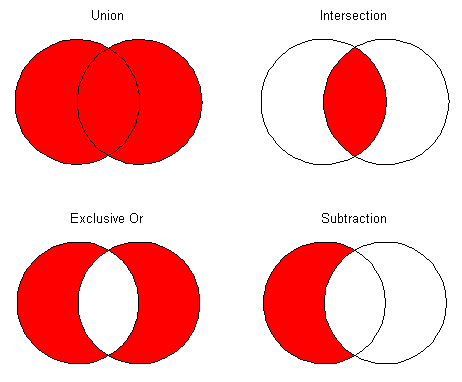
\includegraphics[scale=0.7]{img/venn.png}
\caption{Diagram showing common set operations on two sets \label{venn}}
\end{figure}

See Figure \ref{venn} for a visual.

Suppose we have two sets, of size $m$ and $n$ (let $p=m+n$).  How can we calculate these using HashSets and TreeSets?

\subsection{HashSet}
\begin{enumerate}
\item Union (or): iterate over both sets - $O(p)$.
\item Intersection: iterate over first set, hash the values, determine whether or not in the second set - $O(m)$.
\item Symmetric difference (xor): opposite of intersection - $O(m)$.
\item Subtraction: same as exclusive or, but use only one set - $O(m)$.
\end{enumerate}

\subsection{TreeSets}
\begin{enumerate}
\item Union (or): iterate over both trees, get a set of size $p$, then insert $p$ elements into second tree - $O(m \log n)$.
\item Intersection: iterate first tree, remove elements from second - $O(m \log n)$.
\item Symmetric difference: opposite of intersection - $O(m \log n)$.
\item Subtraction: iterate over first tree, for each find elements in second tree - $O(m \log n)$.
\end{enumerate}

\section{Bit Sets}
We can use bit strings to represent set membership.  Each bit in the string represents either the presence or absence of an element.  For example:
\begin{align*}
\{"mouse","monitor","computer"\}  &\rightarrow 1011 \\
\{"mouse","computer","keyboard"\} &\rightarrow 1101 \\
\{"computer","keyboard"\}         &\rightarrow 1100
\end{align*}
For this kind of representation, the length of the bit string must account for every possible element.  Also, the location of each bit matters; in this example, the first bit is for "computer", second for "keyboard", third for "monitor", fourth for "mouse".

\subsection{Set operations}
Using bitwise operations and a bit string representation of two sets, we can easily implement union, intersection, symmetric difference, and subtraction.

Let $a$ and $b$ be two sets represented by bit strings.  Then:
\begin{itemize}
\item union: $a$ \verb|or| $b$
\item intersection: $a$ \verb|and| $b$
\item symmetric difference: $a$ \verb|xor| $b$
\item subtraction: $a-b$
\end{itemize}

These are all technically $O(n)$, where $n$ is the number of bytes ($a$ and $b$) must be the same length.  However, the growth rate is very slow, even though it is linear.  This is because:

\begin{itemize}
\item For a 64-bit CPU, bitwise operations operate on 64 bits in a single CPU operation.
\item In tree / hash implementations, you have to compare 64 objects with 64 objects, one by one.
\item The simplicity of bit string operations is optimized on the CPU.
\end{itemize}

Technically, these operations are $O(n/w)$, where $w$ is the word size.  In practice, bitwise operations are much faster than other implementations, even if they have lower big-O.

\subsection{Memory}
Bit strings can store $n$ different pieces of data in $n/w$ words - this is about as compact as you can get without compression.

However, note that every possible item in the set must be represented by a bit.  What if sets are very sparse?  For example, two sentences of English words.  There are hundreds of thousands of words, but often sentences only contain a few.  In this case, we have to represent the two sentences using very long bit strings, most of which are 0.  This is not optimal.

\end{document}
